\documentclass[conference]{IEEEtran}
\IEEEoverridecommandlockouts
\usepackage{cite}
\usepackage{amsmath,amssymb,amsfonts}
\usepackage{algorithmic}
\usepackage{graphicx}
\graphicspath{ {./lineplot/} }
\usepackage{textcomp}
\usepackage{xcolor}
\def\BibTeX{{\rm B\kern-.05em{\sc i\kern-.025em b}\kern-.08em
    T\kern-.1667em\lower.7ex\hbox{E}\kern-.125emX}}
\begin{document}

\title{Popularity of Programming languages over the years\\
{\footnotesize \textsuperscript{}Data analysis on most popular programming languages from 2004 to 2022}}


\author{\IEEEauthorblockN{Aryan Singh}
\IEEEauthorblockA{\textit{Department of Computer Science and Engineering} \\
\textit{Meghnad Saha Institute of Technology}\\
Calcutta, India \\
aryansingh_cse2021@gmail.com}
\and
\IEEEauthorblockN{Neeraj P Pillai}
\IEEEauthorblockA{\textit{Department of Computer Science and Engineering} \\
\textit{Meghnad Saha Institute of Technology}\\
Calcutta, India \\
neeraj_p.cse2021@msit.edu.in}
\and
\IEEEauthorblockN{Abdul Basit}
\IEEEauthorblockA{\textit{Department of Computer Science and Engineering} \\
\textit{Meghnad Saha Institute of Technology}\\
Calcutta, India \\
abdul_b.cse2021@msit.edu.in}
\and
\IEEEauthorblockN{Kuntal Barik}
\IEEEauthorblockA{\textit{Department of Computer Science and Engineering} \\
\textit{Meghnad Saha Institute of Technology}\\
Calcutta, India \\
kuntal_b.cse2021@msit.edu.in}
\and
\IEEEauthorblockN{Harshil D Sheth}
\IEEEauthorblockA{\textit{Department of Computer Science and Engineering} \\
\textit{Meghnad Saha Institute of Technology}\\
Calcutta, India \\
hdsheth.cse2021@msit.edu.in}
}

\maketitle

\begin{abstract}
We begin with the age-old and divisive question "Which is the best programming language?". But with a willingness to keep the same number of friends, when we started out with this project!
\end{abstract}

\section{Introduction}
This project is based on data analysis of popular programming languages over the decades
We have used the functionality provided by the Python programming language and libraries built for the same. The libraries used are Pandas, numpy, and Seaborn. The data collected has been categorically sorted into months leading to January 2022. In this project, we have discussed how languages have held up over the years.

\subsection{Primary Categorisation}\label{AA}
We have settled into four primary categorisations : 

\begin{itemize}
\item \textbf{[PP]} The languages which have remained popular over the years.
\item \textbf{[PF]} The languages which are no longer popular.
\item \textbf{[FP]} The languages which have become popular.
\item \textbf{[FF]} Languages that never gained market dominance.
\end{itemize}

\subsection{Secondary Categorisation}
The secondary category are designed to include languages that show  trends that do not necessarily fit into what we have established in the primary categories, secondary categories :
\begin{itemize}
\item "Mid for Life", this category has been named after a popular gen-z slang ''mid'' meaning below average.
\item "Gaining Popularity", this category includes languages that are early in development and are gaining market rapidly.
\end{itemize}

\section{Definitions}
\textbf{Popular:} for a language to be considered popular a minimum of 8% or 8 out of every 100 people must use the language. 

\textbf{Mid:} is a language that never crossed the upper boundary of 7% and a lower boundary of 3%.

\textbf{Bust:} is a language that never gained more than 3% of the dominant market share.

\section{Primary Classification}

\subsection{PP}
The languages which have remained popular over the year. The only language in our data-set that fits with this description of ours is JavaScript.
\begin{itemize}
\item{Javascript}
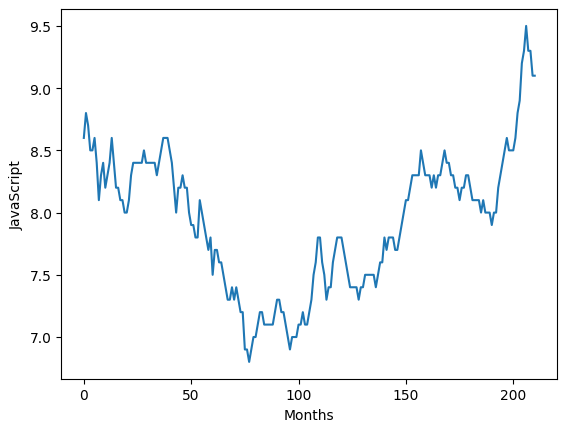
\includegraphics[scale=0.4]{lineplot/javascript.png}
\end{itemize}

\subsection{PF}
The languages which are no longer popular.

\begin{itemize}
\item{Visual Basic}
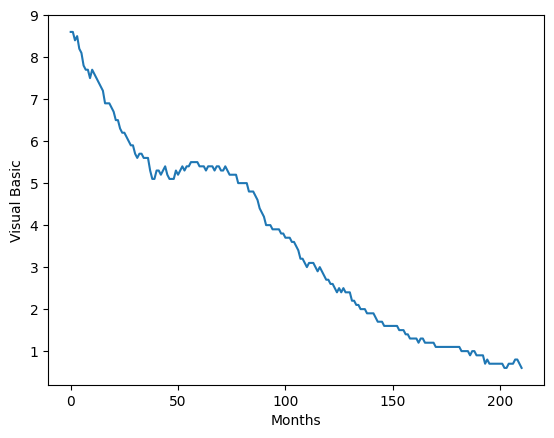
\includegraphics[scale=0.4]{lineplot/visualbasic.png}
\item{PHP}
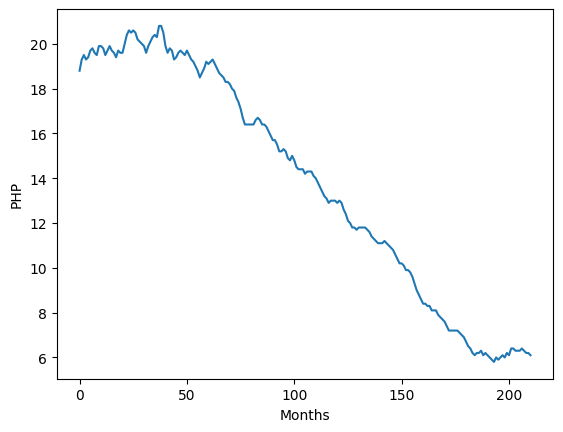
\includegraphics[scale=0.4]{lineplot/php.png}
\item{Perl}
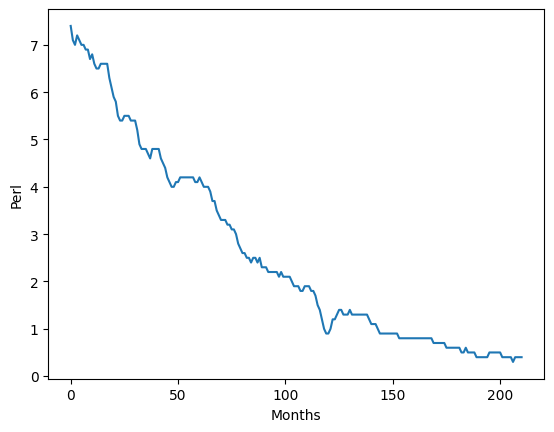
\includegraphics[scale=0.4]{lineplot/perl.png}
\item{Java}
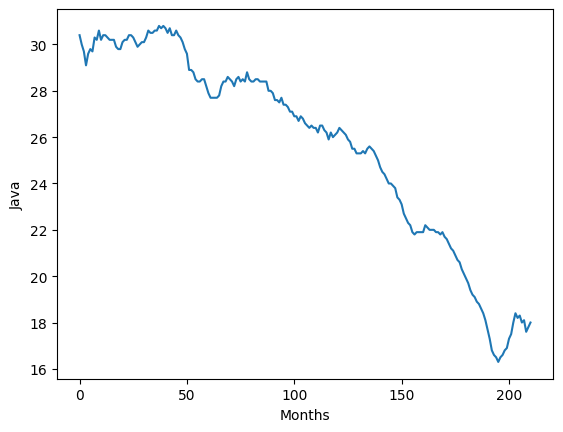
\includegraphics[scale=0.4]{lineplot/java.png}
\end{itemize}

\subsection{FP}
The languages which have become popular. The only language fitting this description of ours is Python.
\begin{itemize}
\item{Python}
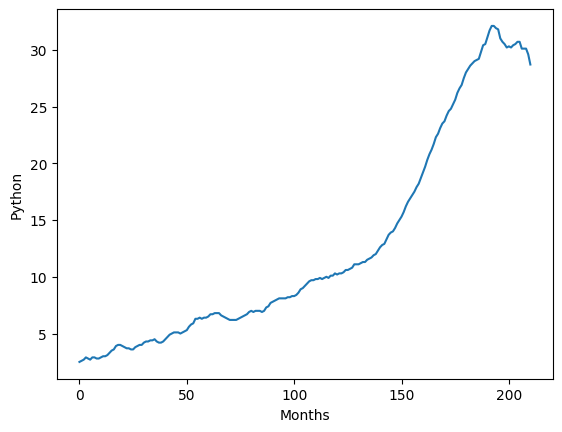
\includegraphics[scale=0.4]{lineplot/python.png}
\end{itemize}

\subsection{FF}
The languages that never gained market dominance

\begin{itemize}
\item{VBA}
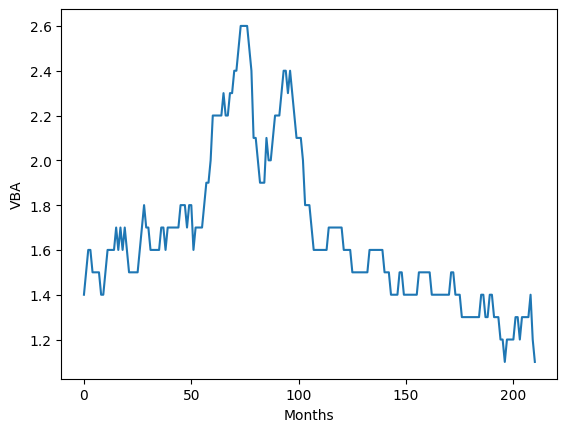
\includegraphics[scale=0.4]{lineplot/vba.png}
\item{Scala}
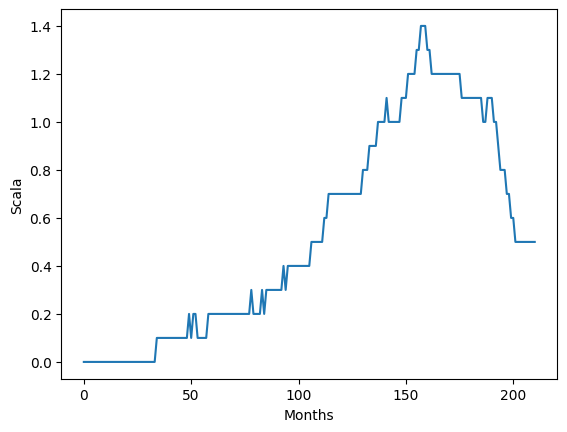
\includegraphics[scale=0.4]{lineplot/scala.png}
\item{Rust}
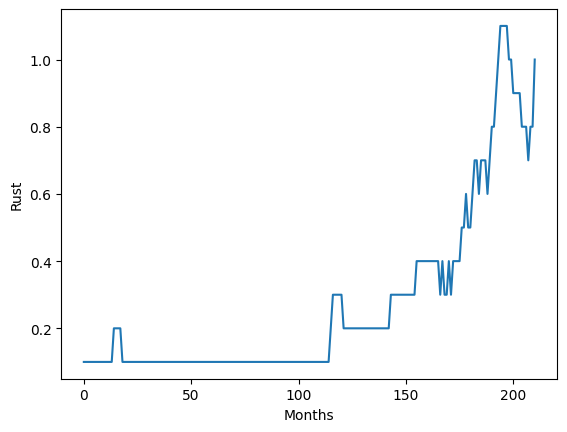
\includegraphics[scale=0.4]{lineplot/rust.png}
\item{Lua}
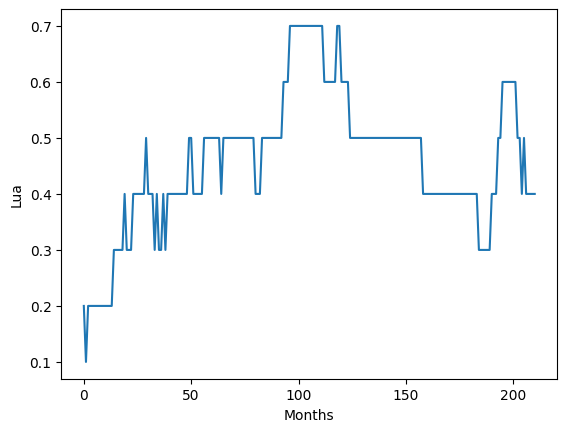
\includegraphics[scale=0.4]{lineplot/lua.png}
\item{Pascal}
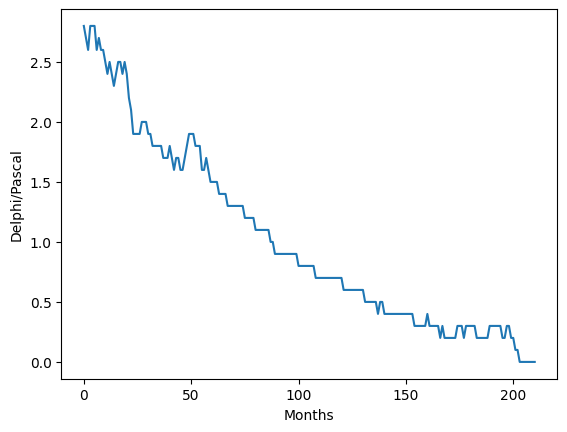
\includegraphics[scale=0.4]{lineplot/pascal.png}
\item{Cobol}
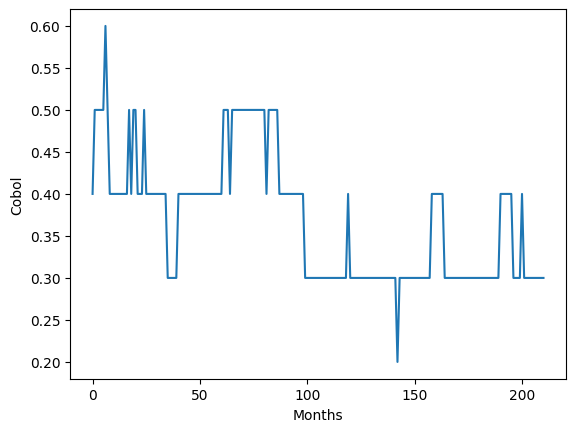
\includegraphics[scale=0.4]{lineplot/cobol.png}
\item{Ada}
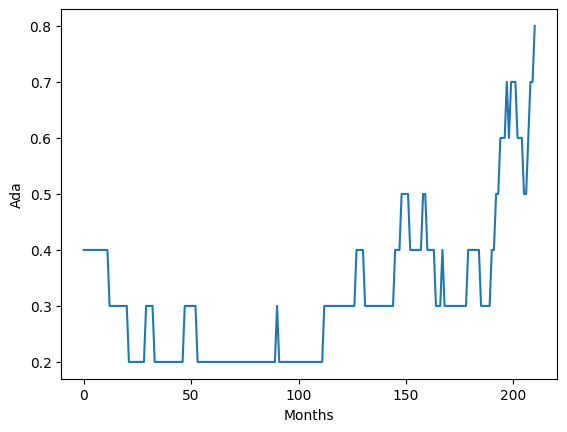
\includegraphics[scale=0.4]{lineplot/ada.png}
\item{Abap}
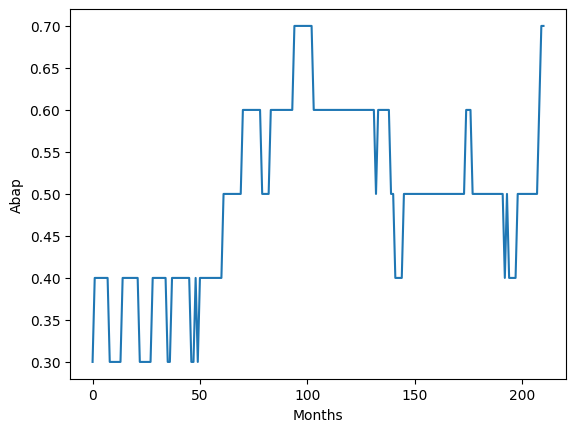
\includegraphics[scale=0.4]{lineplot/abap.png}
\end{itemize}

\section{Secondary Classification}

\subsection{\textit{Mid for life}}
This category has been named after a popular gen-z slang ''mid'' meaning below average.

\begin{itemize}
\item{Swift}
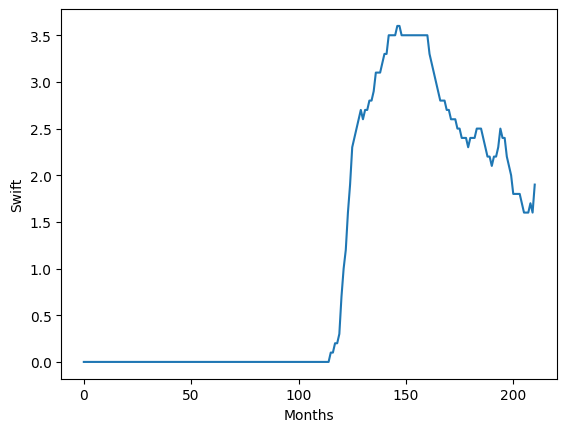
\includegraphics[scale=0.4]{lineplot/swift.png}
\item{Ruby}
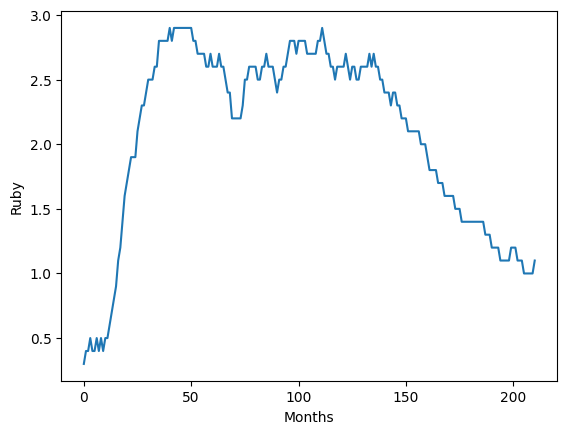
\includegraphics[scale=0.4]{lineplot/ruby.png}
\item{Objective-C}
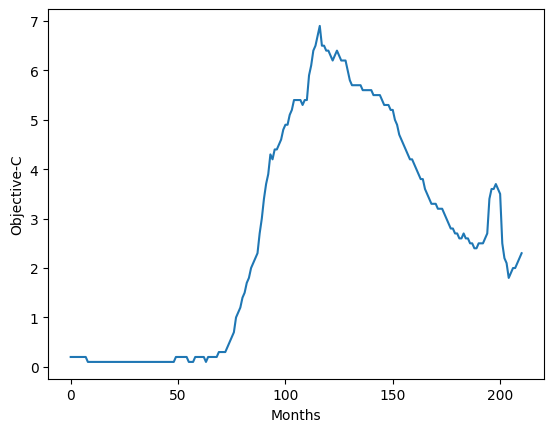
\includegraphics[scale=0.4]{lineplot/objective-c.png}
\item{Matlab}
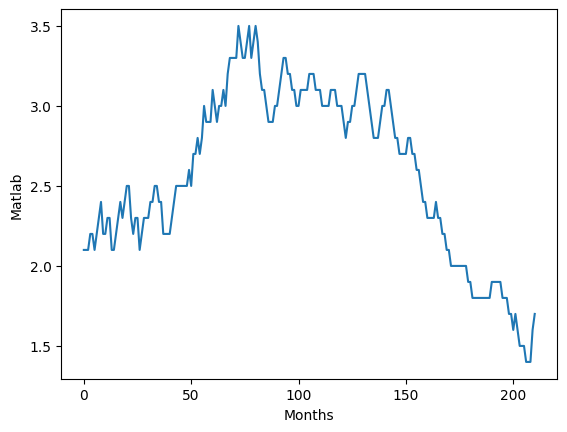
\includegraphics[scale=0.4]{lineplot/matlab.png}
\item{Kotlin}
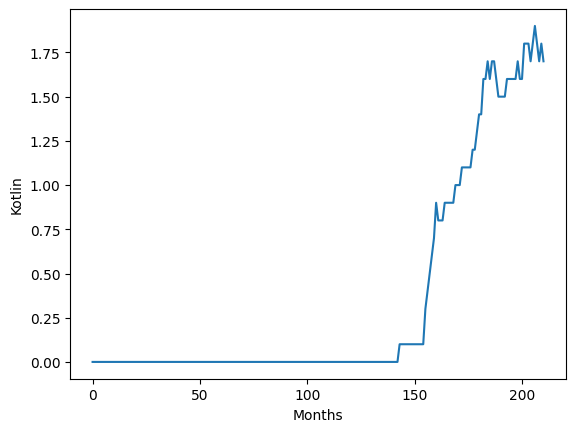
\includegraphics[scale=0.4]{lineplot/kotlin.png}
\item{Julia}
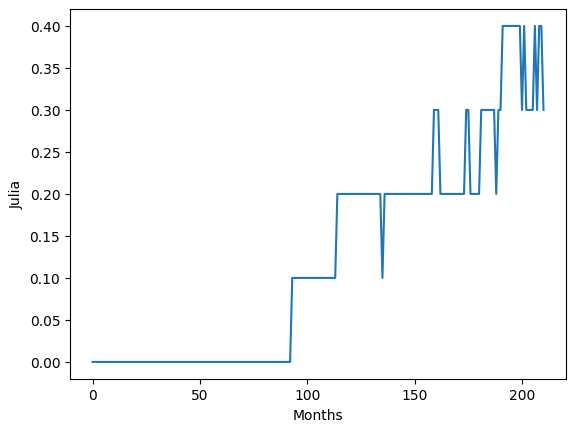
\includegraphics[scale=0.4]{lineplot/julia.png}
\item{Haskell}
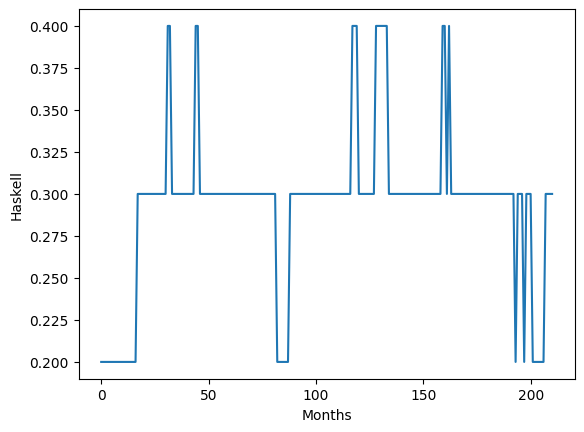
\includegraphics[scale=0.4]{lineplot/haskell.png}
\item{C sharp}
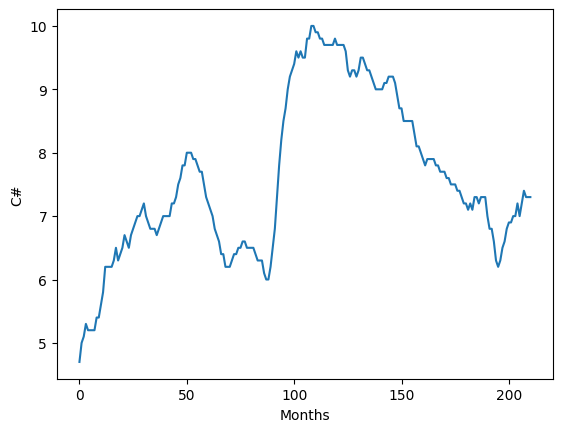
\includegraphics[scale=0.4]{lineplot/c-sharp.png}
\item{C/C++}
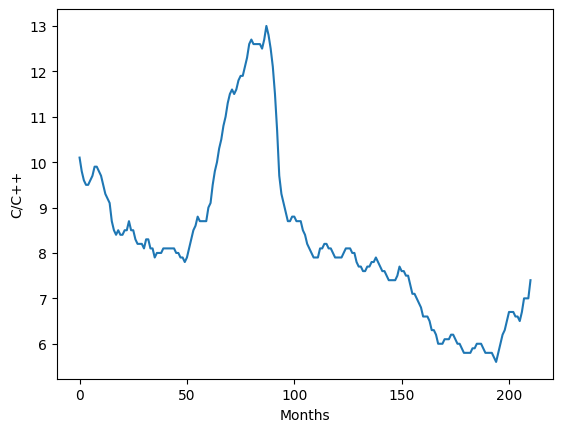
\includegraphics[scale=0.4]{lineplot/ccpp.png}
\end{itemize}

\subsection{\textit{Gaining Popularity}}
This category includes languages that are early in development and are gaining market rapidly.

\begin{itemize}
\item{Typescript}
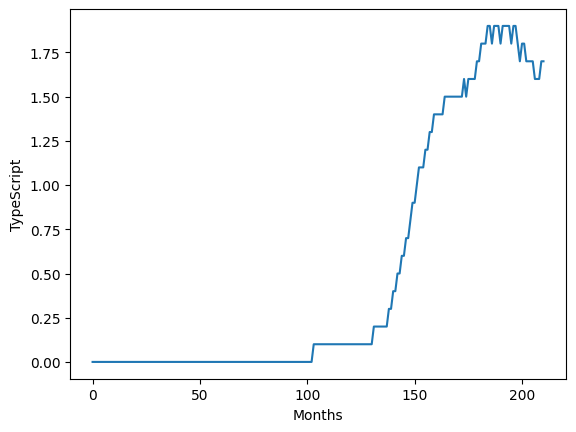
\includegraphics[scale=0.4]{lineplot/typescript.png}
\item{R}
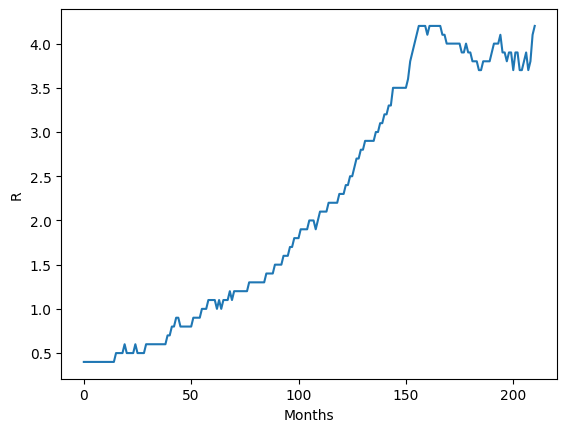
\includegraphics[scale=0.4]{lineplot/r.png}
\item{Groovy}
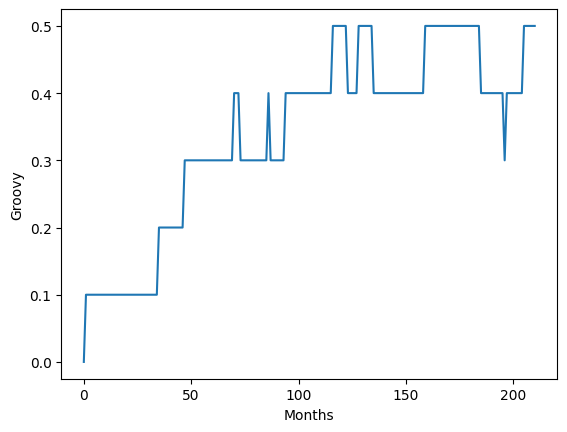
\includegraphics[scale=0.4]{lineplot/groovy.png}
\item{Go}
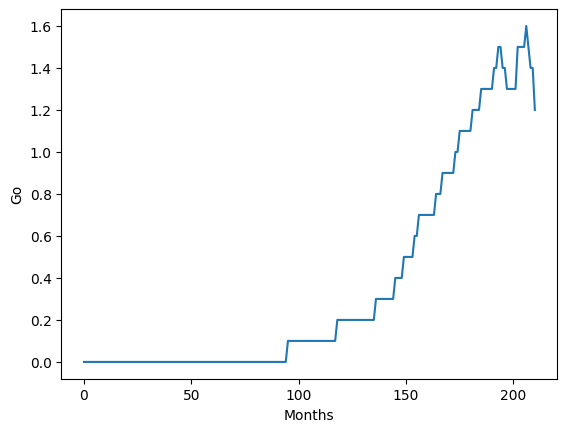
\includegraphics[scale=0.4]{lineplot/go.png}
\item{Dart}
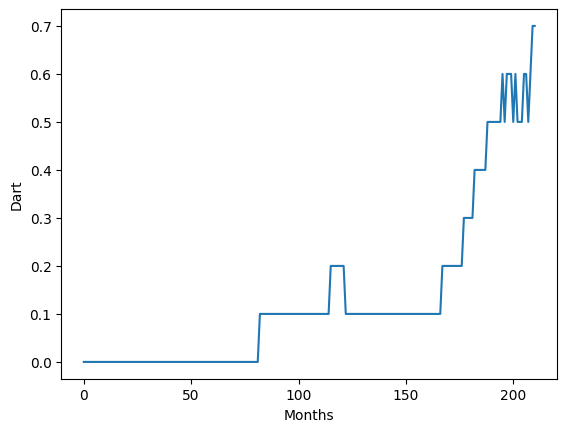
\includegraphics[scale=0.4]{lineplot/dart.png}
\end{itemize}

\subsection{Correlation}
In statistics, correlation or dependence is any statistical relationship, whether causal or not, between two random variables or bivariate data. Although in the broadest sense, "correlation" may indicate any type of association, in statistics it usually refers to the degree to which a pair of variables are linearly related. Familiar examples of dependent phenomena include the correlation between the height of parents and their offspring, and the correlation between the price of a good and the quantity the consumers are willing to purchase, as it is depicted in the so-called demand curve.

Correlations are useful because they can indicate a predictive relationship that can be exploited in practice. For example, an electrical utility may produce less power on a mild day based on the correlation between electricity demand and weather. In this example, there is a causal relationship, because extreme weather causes people to use more electricity for heating or cooling. However, in general, the presence of a correlation is not sufficient to infer the presence of a causal relationship (i.e., correlation does not imply causation). 

In our analysis we have found that Java was the top language till April 2018, starting from July 2004. Then the top spot has been reserved by Python, till the end of our sample size. Seeing this we decided to run a comprehensive analysis of the correlation between python and Java. We have also included their correlation to other languages.

\subsection{Correlation between other languages and Python and Java}
\begin{center}
\begin{tabular}{ c c c }
Languages & Python & Java\\\\
Abap & 0.210543 & -0.275354\\
Ada & 0.677052 & -0.711266\\
C/C++ & -0.702704 & 0.681450\\
C-Sharp & 0.085039 & -0.169606\\
Cobol & -0.514747 & 0.534975\\
Dart & 0.901937 & -0.891201\\
Delphi/Pascal & -0.803821 & 0.842192\\
Go & 0.985374 & -0.957954\\
Groovy & 0.676539 & -0.719915\\
Haskell & 0.028710 & -0.049515\\
Java & -0.983492 & 1.000000\\
JavaScript & 0.385331 & -0.322988\\
Julia & 0.905960 & -0.939636\\
Kotlin & 0.945595 & -0.892701\\
Lua & 0.069608 & -0.154700\\
Matlab & -0.617304 & 0.529346\\
Objective-C & 0.325187 & -0.431106\\
Perl & -0.783993 & 0.826646\\
PHP & -0.943219 & 0.966258\\
Python & 1.000000 & -0.983492\\
R & 0.900140 & -0.933396\\
Ruby & -0.441982 & 0.411585\\
Rust & 0.925995 & -0.916171\\
Scala & 0.733003 & -0.777016\\
Swift & 0.695197 & -0.745004\\
TypeScript & 0.970837 & -0.944515\\
VBA & -0.602485 & 0.588156\\
Visual Basic & -0.870000 & 0.898426\\

\end{tabular}
\end{center}

\end{document}